
Using a linear fit from the energy calibration earlier, we applied this to the $^{133}$Ba data to yield the
plot below.

\begin{figure}[H]
  \begin{center}
    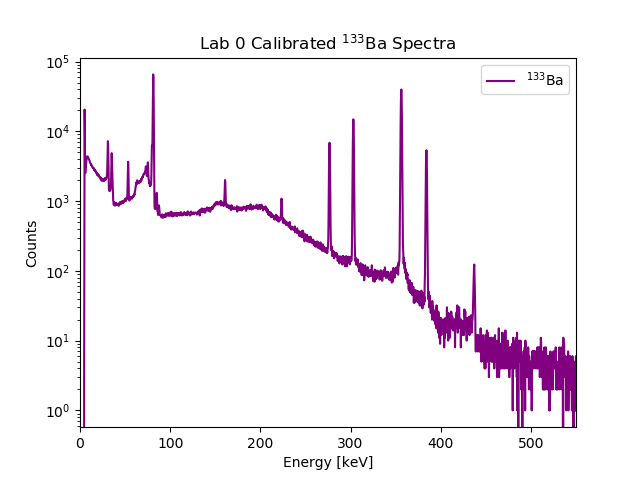
\includegraphics[width=10cm]{ba_calibrated.png}
    \caption{\label{fig:ba133}Calibrated $^{133}$Ba Spectra}
  \end{center}
\end{figure}

The accepted values were then compared against the energy values found thought the energy calibration, calculating the
percent difference between the two.
\\

\begin{tabular}{lll}
\toprule
Calculated Energy [keV] & Accepted Value [keV] & Precent Difference \% \\
\midrule
     81.14525+/-0.00010 &     80.9979+/-0.0011 &      0.1819+/-0.0014 \\
    356.39031+/-0.00005 &    356.0129+/-0.0007 &    0.10601+/-0.00020 \\
      5.10916+/-0.00011 &                 4.47 &     14.2988+/-0.0024 \\
    303.08087+/-0.00006 &    302.8508+/-0.0005 &    0.07597+/-0.00017 \\
     30.92215+/-0.00010 &               32.194 &    3.95059+/-0.00033 \\
    276.70673+/-0.00006 &      275.925+/-0.007 &      0.2833+/-0.0025 \\
    384.16733+/-0.00005 &    383.8485+/-0.0012 &    0.08306+/-0.00031 \\
\bottomrule
\end{tabular}

\\

This comparison shows that the linear fit is good for higher gamma energies but is significantly
degraded for lower energy events.
